% ch0.tex
% This work is licensed under the Creative Commons Attribution-Noncommercial-Share Alike 3.0 New Zealand License.
% To view a copy of this license, visit http://creativecommons.org/licenses/by-nc-sa/3.0/nz
% or send a letter to Creative Commons, 171 Second Street, Suite 300, San Francisco, California, 94105, USA.

\chapter{Instalación de Python}\label{ch:instalacion}

\noindent
Nivel de dificultad:\difl

\begin{citaCap}
``Tempora mutantur nos et mutamur in illis''\\
(Los tiempos cambian, y nosotros cambiamos con ellos)\\
---antiguo proverbio romano
\end{citaCap}

\section{Inmersión}

Bienvenido a Python 3. ¡Vamos a mojarnos! En este capítulo, vas a instalar la versión de Python adecuada para ti.

\section{¿Cuál es la versión adecuada para ti?}

Lo primero que necesitas hacer es instalar Python 3.

Si estás utilizando una sesión en un servidor remoto (posiblemente a través de Internet), el administrador del servidor puede que ya lo haya instalado por ti. Si estás utilizando Linux\footnote{Nota del Traductor: El nombre correcto del sistema operativo Linux es GNU/Linux, no obstante, por comodidad, en este libro se utilizará únicamente Linux para mayor comodidad} en casa, puede que también lo tengas ya instalado, aunque actualmente\footnote{año 2009} la mayor parte de las distribuciones de Linux vienen con Python 2 instalado (como verás en este capítulo, puedes tener simultáneamente más de una versión de Python en tu ordenador sin problemas). En los Mac OS X se incluye una versión de línea de comando de Python 2, pero no Python 3. Microsoft Windows no trae ninguna versión de Python. Pero ¡no te preocupes! siempre puedes instalarlo tú mismo, tengas el sistema operativo que tengas.

La forma más sencilla para comprobar si tienes instalado Python 3 en tu sistema Linux o Mac OS X es abrir un terminal de línea de comandos. Para ello debes hacer lo siguiente:

\begin{itemize}
\item Si estás en Linux, busca en el menú de \codigo{Aplicaciones} un programa denominado \codigo{terminal} (puede estar en un submenú, posiblemente \codigo{Accesorios} o \codigo{Sistema}).
\item Si estás en Mac OS X, existe una aplicación que se llama \codigo{Terminal.app} en la carpeta \codigo{/Aplicaciones/Utilidades/}.
\end{itemize}

Una vez te encuentres en la línea de comando\footnote{También conocido como el ``prompt''}, teclea \codigo{python3} (en minúsculas y sin espacios) y observa lo que sucede. En mi sistema Linux, Python 3 ya está instalado, por lo que el resultado de ejecutar este comando hace que el terminal entre en la \emph{consola\footnote{En inglés ``shell''} interactiva de Python}.
\begin{listing}
\begin{verbatim}
jmgaguilera@acerNetbook-jmga:~$ python3
Python 3.0.1+ (r301:69556, Apr 15 2009, 15:59:22) 
[GCC 4.3.3] on linux2
Type "help", "copyright", "credits" or "license" for more information.
>>> 
\end{verbatim}
\end{listing}

(Para salir de la consola interactiva de Python escribe \codigo{exit()} y pulsa la tecla \codigo{INTRO}.)

Al ejecutar esta misma sentencia \codigo{python3} en un ordenador Linux que no tenga instalado Python 3 el mensaje que se obtendrá será parecido al siguiente:

\begin{listing}
\begin{verbatim}
jmgaguilera@acerNetbook-jmga:~$ python3
bash: python3: orden no encontrada
jmgaguilera@acerNetbook-jmga:~$ python3
\end{verbatim}
\end{listing}

Bueno, volviendo ahora a la pregunta sobre cuál es la versión de Python 3 apropiada para ti, queda claro que es aquella que se ejecute en el ordenador que tengas.

Para conocer cómo instalar Python 3, continúa leyendo en el apartado que corresponda a tu sistema operativo.

\section{Instalación en Microsoft Windows}

Windows se ejecuta actualmente en dos plataformas diferentes: 32 y 64 bits. Asimismo, existen diferentes \emph{versiones} de Windows ---XP, Vista, Windows 7--- y Python 3 funciona en todas ellas. Es más importante, con vistas a la instalación, la distinción que existe entre los dos tipos de arquitecturas. Si no sabes de qué tipo es la arquitectura de tu ordenador, lo más probable es que sea de 32 bits.

Visita \href{http://python.org/download/}{python.org/download/} para descargar la aplicación de instalación de Python 3 que sea correcta para para la arquitectura de tu ordenador. Las posibilidades serán parecidas a:

\begin{itemize}
\item \textbf{Python 3.*.* x86 Windows installer} (Windows binary --- does not include sources)
\item \textbf{Python 3.*.* AMD64 Windows installer} (Windows AMD64 binary --- does not include sources)
\end{itemize}

La descarga exacta varía en función de las actualizaciones. Por eso he puesto asteriscos en lugar del número de versión. Deberías instalar siempre la última versión disponible de Python 3.x a menos que tengas alguna razón importante para no hacerlo.

\begin{figure}[!h]
  \begin{center}
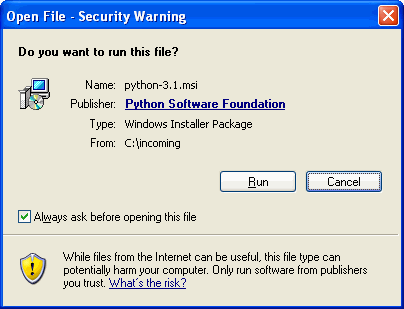
\includegraphics[width=0.5\textwidth]{winInstalacion1.png}
\caption{Advertencia al inicio}\label{fig01}
  \end{center}
\end{figure}

Cuando la descarga finalize, pulsa (doble click) sobre el fichero \codigo{.msi} que has descargado. Windows mostrará una alerta de seguridad (figura~\ref{fig01}) para avisarte de que estás intentando ejecutar un fichero que instalará cosas en tu ordenador. El fichero instalador de Python está firmado electrónicamente por la \href{http://www.python.org/psf/}{\emph{Python Software Foundation}}, que es la organización sin ánimo de lucro que supervisa el desarrollo de Python. ¡No aceptes imitaciones!

Pulsa el botón \codigo{Run} o \codigo{Ejecutar}\footnote{dependerá del idioma en el que se encuentre tu sistema operativo} para que se inicie la ejecución del programa instalador de Python.

\begin{figure}[!h]
 \begin{center}
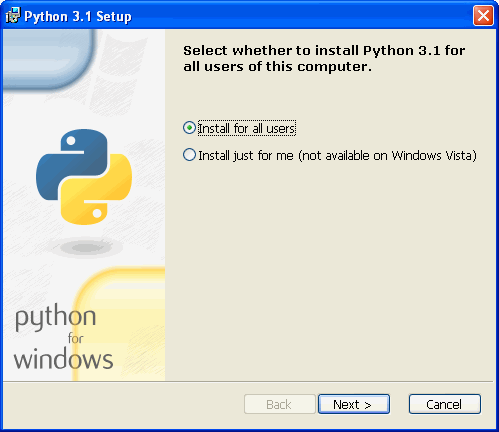
\includegraphics[width=0.5\textwidth]{winInstalacion2.png}
\caption{Tipo de instalación}\label{fig02}
  \end{center}
\end{figure}

Lo primero que pide el programa instalador (figura~\ref{fig02}) es que le indiques si quieres instalar Python 3 para todos los usuarios del ordenadores o únicamente para ti. Por defecto aparece seleccionada la opción ``Instalar para todos los usuarios'', que es la mejor opción, a no ser que tengas una buena razón para no hacerlo\footnote{Una posible razón por la podrías querer instalarlo únicamente para tu usuario es que estuvieras instalando Python en el ordenador de la empresa y no tengas permisos de administrador en tu cuenta de usuario. Pero en ese caso, ¿qué haces instalando Python sin permiso del administrador de tu empresa? A mí no me metas en problemas, eso es cosa tuya.}.

Cuando hayas seleccionado la opción deseada, pulsa el botón \codigo{Next} o \codigo{Siguiente} para continuar con la instalación.

Lo siguiente que pedirá el instalador (figura~\ref{fig03}) es que le digas el directorio de instalación. El valor por defecto para todas las versiones de Python 3.1.x es \codigo{C:$\backslash$Python31$\backslash$}, que es un valor adecuado para la mayoría de los usuarios. Salvo que tengas una razón específica para cambiarlo, como por ejemplo, que mantengas una unidad separada para la instalación de aplicaciones, puedes usar este directorio para instalar Python.

Para cambiar el directorio de instalación, puedes utilizar las opciones de pantalla o, simplemente, teclear el directorio deseado (con el path completo) en la caja de texto.

\begin{figure}[!h]
  \begin{center}
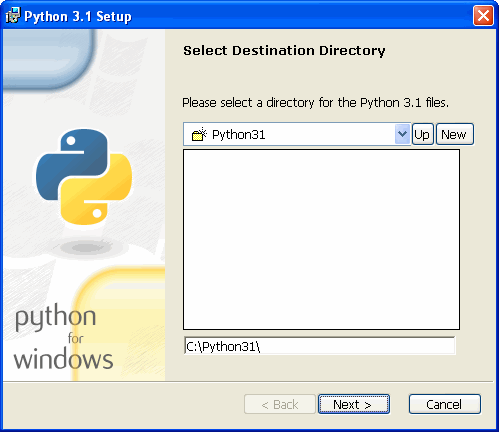
\includegraphics[width=0.5\textwidth]{winInstalacion3.png}
\caption{Directorio de instalación}\label{fig03}
  \end{center}
\end{figure}

Puedes instalar Python en el disco duro en el lugar que desees.

Cuando hayas finalizado, pulsa el botón \codigo{Next} o \codigo{Siguiente} para continuar.

\begin{figure}[!h]
  \begin{center}
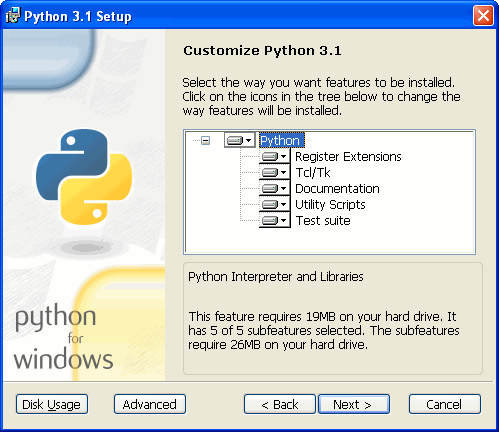
\includegraphics[width=0.5\textwidth]{winInstalacion4.png}
\caption{Selección de elementos a instalar}\label{fig04}
  \end{center}
\end{figure}

La siguiente pantalla (figura~\ref{fig04}) parece más compleja, pero en realidad no lo es. Como pasa con otros muchos instaladores, te ofrece la opción de que selecciones qué cosas concretas quieres instalar. Puedes instalar todos los componentes de Python 3, y si el espacio en disco es justo, puedes excluir ciertos componentes.

\begin{itemize}
\item \textbf{Registrar las extensiones}. Si seleccionas esta opción, el instalador modificará la configuración de Windows para que te permita ejecutar los scripts\footnote{ficheros que contienen sentencias de Python, que normalmente tienen la extensión \codigo{.py}} de Python con solo hacer doble click sobre el fichero. Esta opción no necesita de espacio en disco, por lo que no tiene mucho sentido no marcarla.
\item \textbf{Tcl$\backslash$Tk} es la librería gráfica que utiliza la consola de Python. La usaremos a lo largo de todo el libro, por lo que es muy recomendable que la mantengas entre los componentes a instalar.
\item \textbf{Documentación} instala un fichero de ayuda que contiene gran parte de la información que se encuentra en \href{http://docs.python.org/}{docs.python.org}. Es recomendable instalar esta opción cuando es previsible que no dispongas de conexión permanente a Internet.
\item \textbf{Scripts de utilidades}. Estos scripts incluyen diversas utilidades, entre ellas el script \codigo{2to3.py} sobre el que hablaremos más adelante. Es necesaria si vas a migrar código de Python 2 a Python 3. Si no dispones de código para migrar puedes saltarte esta opción.
\item \textbf{Suite de pruebas.} Es una colección de scripts que se utilizan para probar el buen funcionamiento del intérprete de Python. En este libro no lo vamos a usar, yo no lo he usado jamás en el largo tiempo que llevo programando en Python. Es totalmente opcional su instalación.
\end{itemize}

\begin{figure}[!h]
  \begin{center}
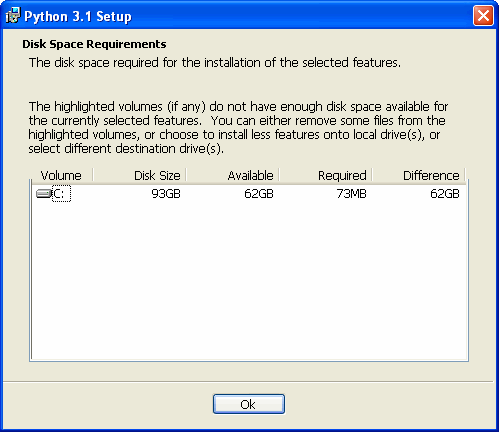
\includegraphics[width=0.5\textwidth]{winInstalacion5.png}
\caption{Espacio libre}\label{fig05}
  \end{center}
\end{figure}

Si no estás seguro de cuando espacio en disco tienes libre, pulsa el botón \codigo{Disk Usage}. El instalador te mostrará las unidades de disco (figura~\ref{fig05}) y el espacio libre disponible en cada una de ellas, así como el espacio que quedará después de la instalación.

Cuando termines la comprobación, pulsa el botón \codigo{OK} para volver a la pantalla anterior.

Si decides excluir alguna opción (figura~\ref{fig06}), selecciona el botón desplegable que aparece a la izquierda del texto de la opción y selecciona \codigo{Entire feature will be unavailable}. Por ejemplo, si excluyes la suite de pruebas ahorrarás 7908 KBytes de espacio en disco.

\begin{figure}[!h]
  \begin{center}
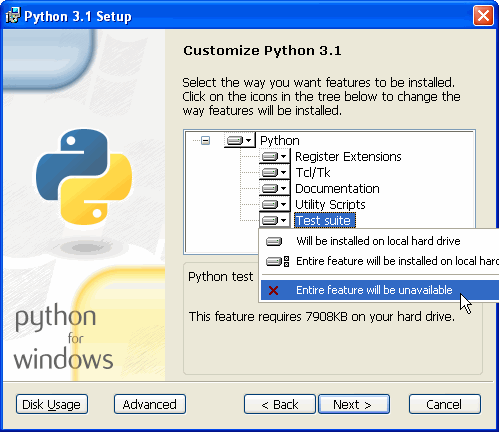
\includegraphics[width=0.5\textwidth]{winInstalacion6.png}
\caption{Excluir una opción}\label{fig06}
  \end{center}
\end{figure}

Pulsa el botón \codigo{Next} para confirmar tu selección de opciones.


\begin{figure}[!h]
  \begin{center}
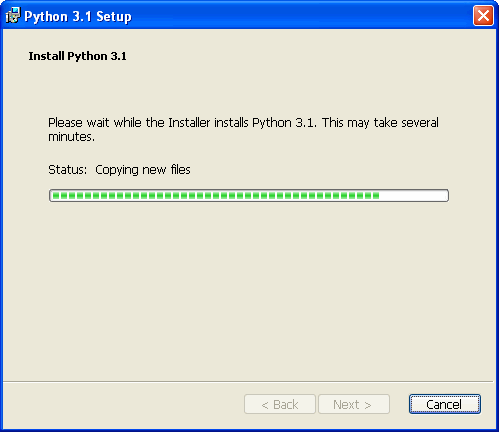
\includegraphics[width=0.5\textwidth]{winInstalacion7.png}
\caption{Instalación}\label{fig07}
  \end{center}
\end{figure}

El instalador copiará todos los ficheros (figura~\ref{fig07} al directorio de destino que hayas seleccionado (Suele ser tan rápido, que tuve que probarlo tres veces antes de conseguir sacar una ``foto'' de la pantalla mostrándolo).
 
\begin{figure}[!h]
  \begin{center}
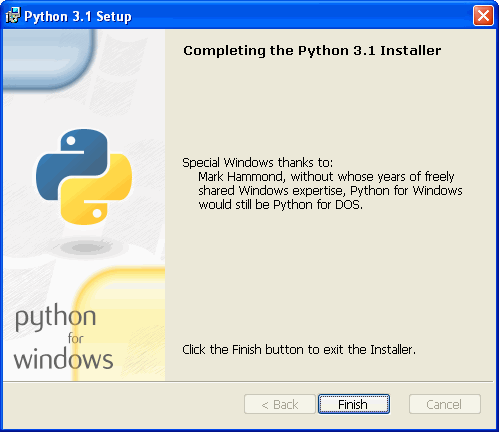
\includegraphics[width=0.5\textwidth]{winInstalacion8.png}
\caption{Instalación completada}\label{fig08}
  \end{center}
\end{figure}

Por último, pulsa el botón \codigo{Finish} para salir del instalador (figura~\ref{fig08}).


\begin{figure}[!h]
  \begin{center}
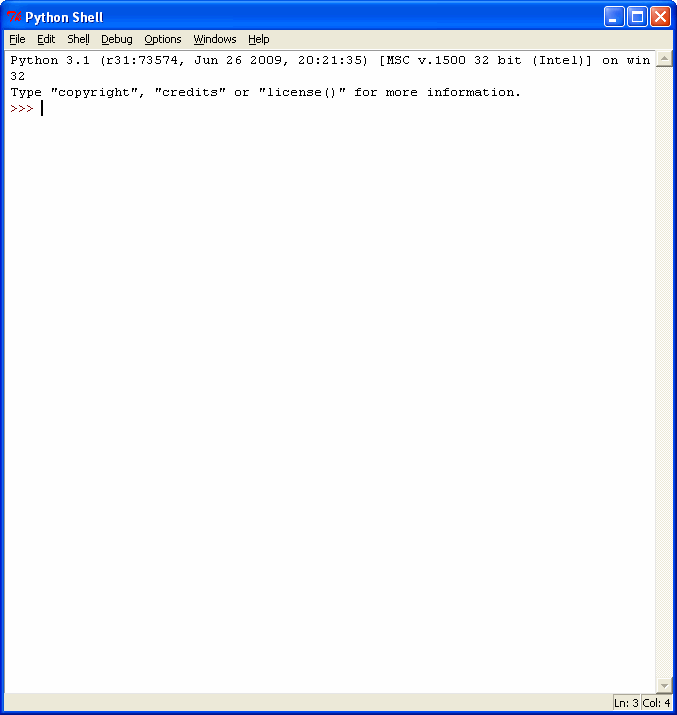
\includegraphics[width=0.5\textwidth]{winInstalacion9.png}
\caption{Instalación completada}\label{fig09}
  \end{center}
\end{figure}

Si ahora buscas en el menú de \codigo{Inicio}, deberías encontrar un nuevo elemento denominado \codigo{Python 3.1}. Dentro de esta nueva opción de menú encontrarás dos programas denominados \codigo{Python} e \codigo{IDLE}. Selecciona uno de estos dos elementos para ejecutar la consola interactiva de Python (figura~\ref{fig09}).

Continúa en el apartado~\ref{sec:shell}

\section{Instalación en un Mac OS X}

Todos los ordenadores Apple Macintosh modernos utilizan procesadores de Intel\footnote{Como la mayoría de ordenadores con Windows} Los Macintosh antiguos utilizaban procesadores Power PC. No es necesario que conozcas esta diferencia puesto que únicamente existe un instalador para todos los tipos de Macs.

Visita \href{http://python.org/download/}{python.org/download/} para descargar la aplicación de instalación de Python 3 para Mac. Debes buscar un enlace cuyo nombre sea algo así como \textbf{Mac Installer Disk Image (3.*.*}. El número de versión puede variar, pero asegúrate de descargar una versión de Python 3 y no de Python 2.


\begin{figure}[!h]
  \begin{center}
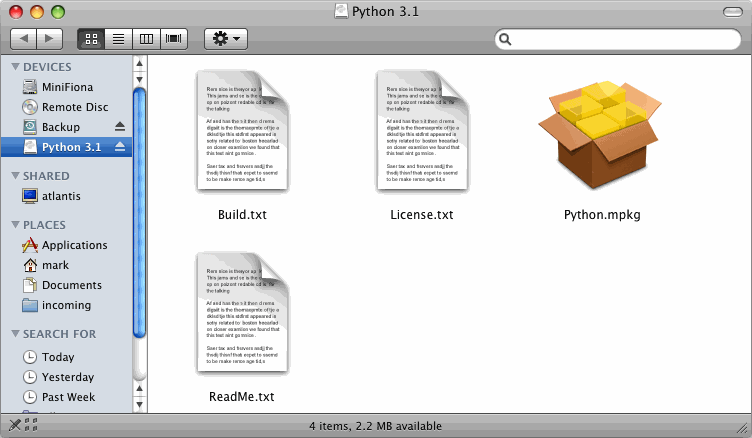
\includegraphics[width=0.5\textwidth]{macInstalacion0.png}
\caption{Finder: contenido de la imagen de disco}\label{figm00}
  \end{center}
\end{figure}

Tu navegador debería montar de forma automática esta imagen de disco y abrir una ventana de \codigo{Finder} para mostrarte el contenido de la imagen. Si no fuese así, deberás buscar la imagen de disco en el directorio de descargas y hacer doble click sobre ella para que se cargue. El nombre de la imagen de disco será algo así como \codigo{python-3-1.dmg}. Una vez tengas visible en pantalla el contenido de la imagen de disco (figura~\ref{figm00}), podrás observar que contiene varios ficheros de texto \codigo{(Build.txt, License.txt, ReadMe.txt)}, y el el fichero del paquete de instalación \codigo{Python.mpkg}.

Haz doble click con el cursor sobre el fichero de instalación \codigo{Python.mpkg} para iniciar el instalador de Python para Mac.

\begin{figure}[!h]
  \begin{center}
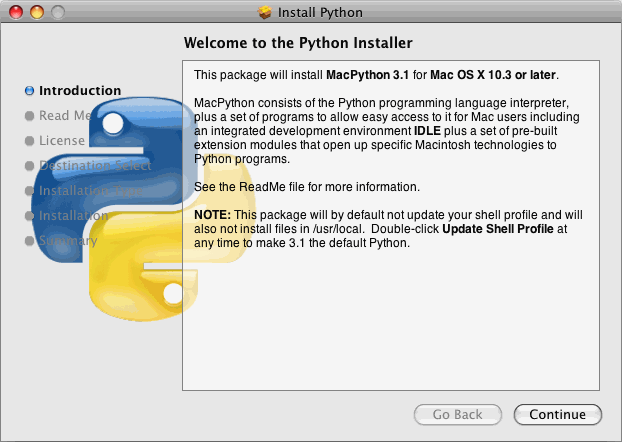
\includegraphics[width=0.5\textwidth]{macInstalacion1.png}
\caption{Bienvenida a la instalación}\label{figm01}
  \end{center}
\end{figure}

La primera página (figura~\ref{figm01}) que muestra el programa de instalación describe de forma concisa qué es Python, y remite al fichero \codigo{ReadMe.txt} (que seguramente no te leíste ¿verdad?) por si deseas conocer más detalles.

Pulsa el botón \codigo{Continue} para avanzar en la instalación.

\begin{figure}[!h]
  \begin{center}
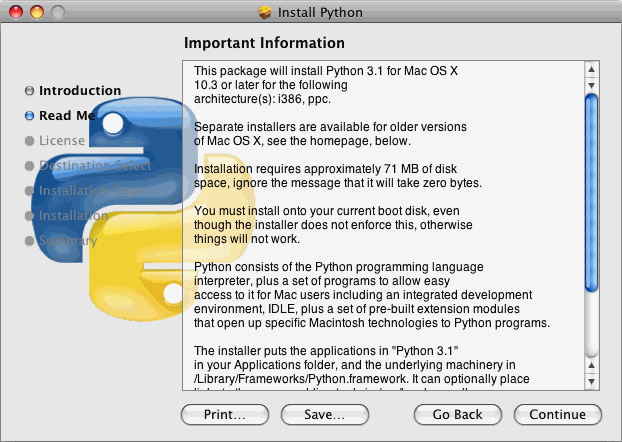
\includegraphics[width=0.5\textwidth]{macInstalacion2.png}
\caption{Información importante}\label{figm02}
  \end{center}
\end{figure}

La siguiente pantalla (figura~\ref{figm02}) muestra información importante: Python necesita que tengas instalado Mac OS X 10.3 o superior. Si estás ejecutando una versión de Mac OS X 10.2 o anterior, deberías actualizar tu ordenador a última versión. Una de las razones más convincentes, es que Apple ya no proporciona actualizaciones de seguridad para tu versión del sistema operativo, por lo que tu ordenadores está en riesgo cada vez que está conectado a Internet. Otra razón, no menos convincente, es que no puedes ejecutar Python 3.

Pulsa el botón \codigo{Continue} para avanzar en la instalación.

\begin{figure}[!h]
  \begin{center}
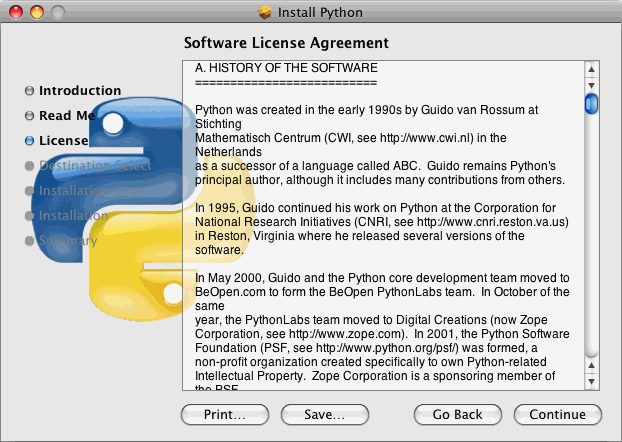
\includegraphics[width=0.5\textwidth]{macInstalacion3.png}
\caption{Licencia}\label{figm03}
  \end{center}
\end{figure}

Como todos los buenos instaladores, lo siguiente que el instalador de Python muestra es la pantalla de aceptación de la licencia (figura~\ref{figm03}). Python es Open Source (software de fuentes abiertas) cuya licencia cuenta con la aprobación de \href{http://opensource.org/licenses/}{la iniciativa de Código Abierto}. Python cuenta con un cierto número de propietarios y patrocinadores a lo largo de su historia, cada uno de los cuales ha dejado su marca en la licencia. Pero el resultado final es este: Python es Código Abierto, y puedes usarlo en cualquier plataforma, para lo que desees, sin necesidad de pagar ningún canon, ni obligación, ni nada a cambio.

Pulsa el botón \codigo{Continue} de nuevo para avanzar en la instalación.

\begin{figure}[!h]
  \begin{center}
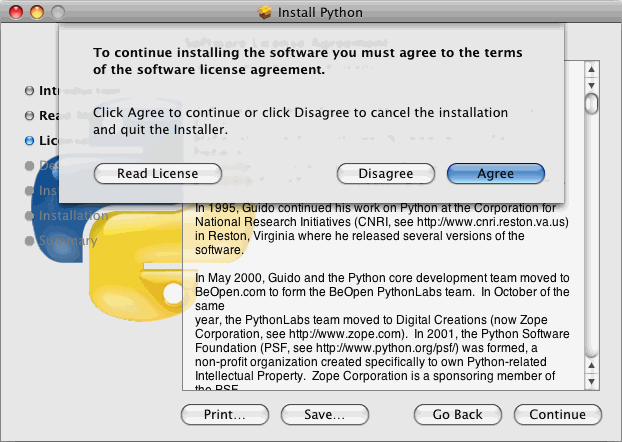
\includegraphics[width=0.5\textwidth]{macInstalacion4.png}
\caption{Aceptación de la Licencia}\label{figm04}
  \end{center}
\end{figure}

Debido a las peculiaridades del proceso de instalación estándar de Apple, es necesario que aceptes la licencia (figura~\ref{figm04}) para que el instalador te permita continuar. Puesto que Python es Código Abierto, en realidad estás aceptando una licencia que te garantiza derechos adicionales, en lugar de quitártelos.

Pulsa el botón \codigo{Agree} para continuar.

La siguiente pantalla (figura~\ref{figm05}) te permite modificar la ubicación en la que se efectuará la instalación. \textbf{Debes} instalar Python en el disco de arranque, pero debido a ciertas limitaciones en el instalador, éste no te obliga a ello, por lo que ¡ten cuidado!. En realidad, yo nunca he tenido la necesidad de cambiar la ubicación de instalación, por ello, salvo causa justificada, acepta la ubicación sugerida por el instalador.

\begin{figure}[!h]
  \begin{center}
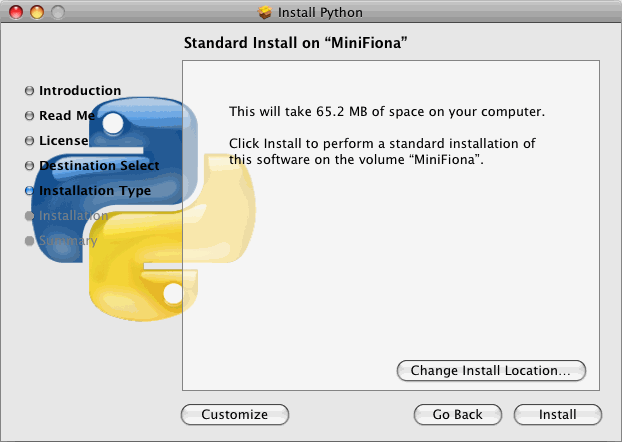
\includegraphics[width=0.5\textwidth]{macInstalacion5.png}
\caption{Selección de la ubicación}\label{figm05}
  \end{center}
\end{figure}

Desde esta pantalla también puedes modificar la instalación con el fin de que no se instalen algunas funcionalidades. Si quieres hacer esto pulsa el botón \codigo{Customize}, en caso contrario pulsa el botón \codigo{Instalar}.

\begin{figure}[!h]
  \begin{center}
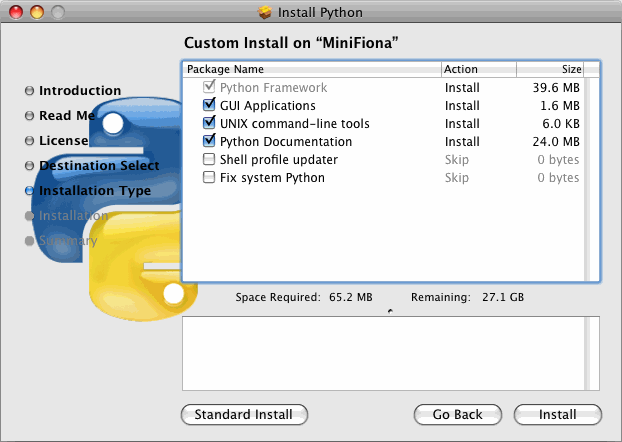
\includegraphics[width=0.5\textwidth]{macInstalacion6.png}
\caption{Personalización de la instalación}\label{figm06}
  \end{center}
\end{figure}

Si eliges una instalación personalizada (has pulsado el botón \codigo{Customize}), el instalador te muestra (figura~\ref{figm06}) una pantalla con una lista de características:

\begin{itemize}
\item \textbf{Python Framework}. Es el núcleo de Python, por lo que está seleccionado y deshabilitado con el fin de que no puedas cambiarlo.
\item \textbf{Aplicaciones GUI} incluye \codigo{IDLE}, la consola interactiva gráfica de Python que usaremos a lo largo de todo el libro. Te recomiendo encarecidamente que mantengas esta opción seleccionada.
\item \textbf{Herramientas de línea de comandos}, que incluyen la aplicación \codigo{python3}. También te recomiendo que mantegas esta opción seleccionada.
\item \textbf{Documentación de Python}, que contiene mucha de la información disponible en \href{http://docs.python.org/}{docs.python.org}. Muy recomendables si tienes previsto estar desconectado de Internet.
\item \textbf{Actualizador del perfil de la consola}, que controla si actualizas tu perfil de consola (utilizado por la aplicación \codigo{Terminal.app}) con el fin de que la versión de Python que estás instalando se encuentre en el camino de búsqueda de la consola. Para los propósitos de este libro, esta opción no es necesario que la instales.
\item \textbf{Actualizar la versión de Python del sistema}. Esta opción no debería modificarse. Le dice a tu ordenador Mac que utilice Python 3 como versión por defecto para todos los scripts, incluido aquellos que vienen con el sistema operativo. Seleccionar esta opción podría producir efectos muy negativos en tu sistema, puesto que la mayor parte de los scripts del sistema operativo están escritos para Python 2, y pueden fallar en Python 3.
\end{itemize}

Pulsa el botón \codigo{Install} para continuar.

\begin{figure}[!h]
  \begin{center}
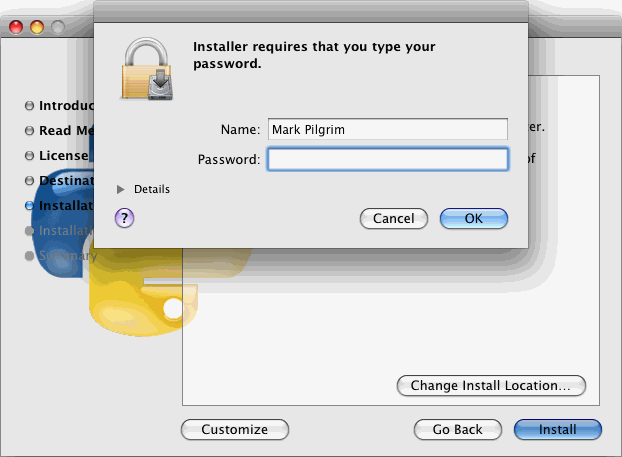
\includegraphics[width=0.5\textwidth]{macInstalacion7.png}
\caption{Solicitando derechos administrativos}\label{figm07}
  \end{center}
\end{figure}

Debido a que el instalador copia archivos binarios en \codigo{/usr/local/bin/}, antes de iniciar dicha copia se solicitan permisos de administrador mediante una pantalla (figura~\ref{figm07}) en la que hay que teclear la clave del administrador del sistema. No es posible instalar Python en Mac sin disponer de las credenciales de administrador.

Pulsa el botón \codigo{OK} para comenzar la instalación.

\begin{figure}[!h]
  \begin{center}
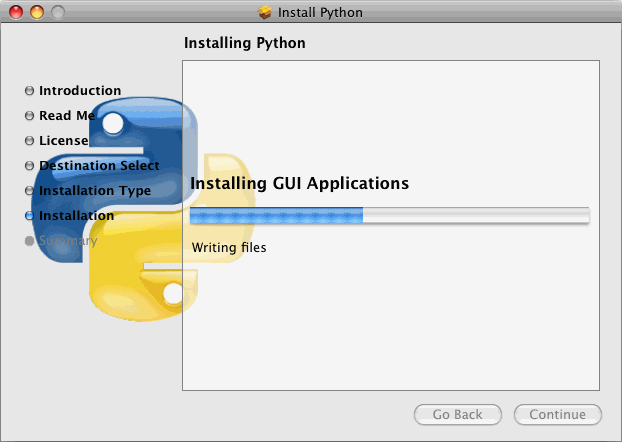
\includegraphics[width=0.5\textwidth]{macInstalacion8.png}
\caption{Instalación}\label{figm08}
  \end{center}
\end{figure}

El instalador mostrará una barra de progreso (figura~\ref{figm08}) mientras se instalan las funcionalidades que hayas seleccionado.

\begin{figure}[!h]
  \begin{center}
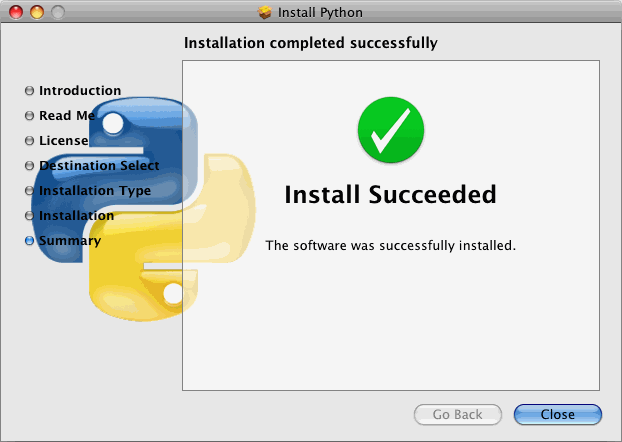
\includegraphics[width=0.5\textwidth]{macInstalacion9.png}
\caption{Fin de la instalación}\label{figm09}
  \end{center}
\end{figure}

Si todo va bien, el instalador mostrará en pantalla (figura~\ref{figm09}) una marca verde para indicar que la instalación de ha completado satisfactoriamente.

Pulsa el botón \codigo{Close} para salir del instalador.

\begin{figure}[!h]
  \begin{center}
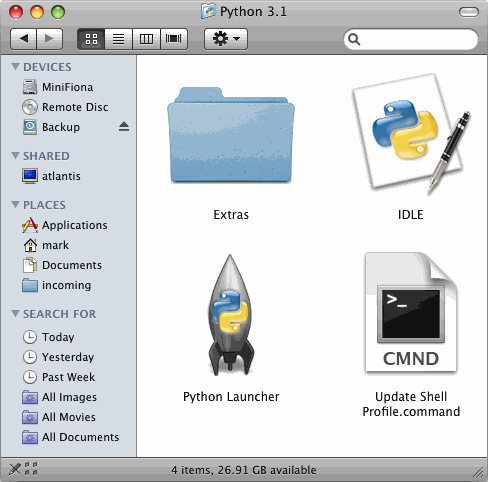
\includegraphics[width=0.5\textwidth]{macInstalacion10.png}
\caption{Carpeta Python}\label{figm010}
  \end{center}
\end{figure}

Si no has cambiado la ubicación de la instalación, \codigo{Python 3.1.*} se habrá instalado en una carpeta denominada \codigo{Python 3.1} (figura~\ref{figm010}) dentro de la carpeta \codigo{/Aplications}. El elemento más importante en ella es \codigo{IDLE}, que es la consola gráfica interactiva de Python.

Haz doble click con el cursor sobre \codigo{IDLE} para ejecutar la consola de Python.

\begin{figure}[!h]
  \begin{center}
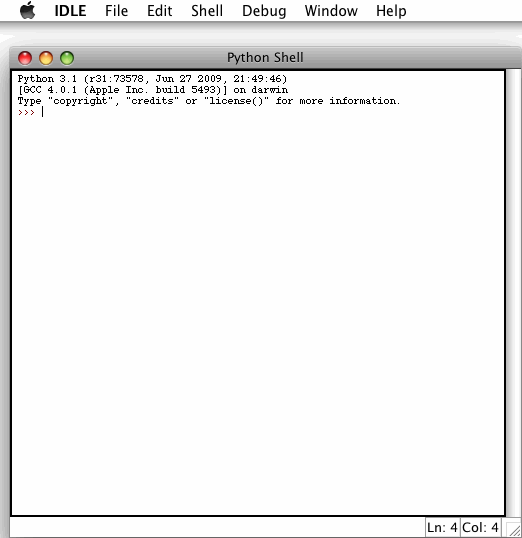
\includegraphics[width=0.5\textwidth]{macInstalacion11.png}
\caption{Consola gráfica}\label{figm011}
  \end{center}
\end{figure}

La mayor parte del tiempo la pasarás explorando Python mediante el uso de esta consola (figura~\ref{figm011}). Los ejemplos de este libro asumen que eres capaz de ejecutar esta consola en todo momento.

Continúa en el apartado~\ref{sec:shell}

\section{Instalación en Ubuntu Linux}

Las diferentes distribuciones existentes hoy día de Linux suelen disponer de vastos repositorios de aplicaciones listas para instalar de forma sencilla. Los detalles exactos varían en función de la distribución de Linux. En Ubuntu Linux, la forma más sencilla de instalar Python 3 consiste en usar la opción \codigo{Añadir y quitar...} del menú de \codigo{Aplicaciones} (figura~\ref{figu00}).

\begin{figure}[!h]
  \begin{center}
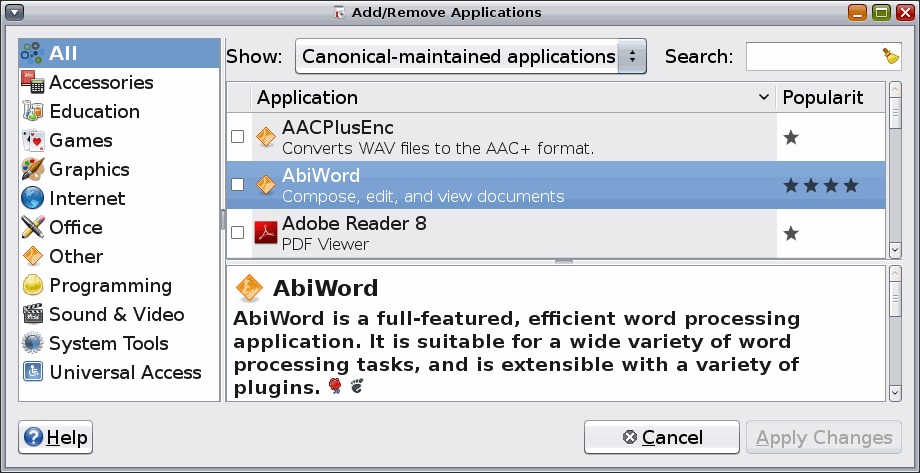
\includegraphics[width=0.6\textwidth]{ubuInstalacion0.png}
\caption{Añadir/Quitar aplicaciones}\label{figu00}
  \end{center}
\end{figure}

Cuando ejecutas por primera vez el programa para \codigo{Añadir/Quitar} aplicaciones, se muestra una lista de aplicaciones preseleccionadas en diferentes categorías. Algunas ya se encuentran instaladas en tu ordenador, pero la mayoría no. Puesto que este repositorio consta de más de 10.000 aplicaciones, encontrar la que se desea puede ser difícil, para facilitar la labor es posible aplicar diferentes filtros que limitan las aplicaciones que se muestran en la lista de pantalla. El filtro por defecto es ``aplicaciones mantenidas por Canonical'' que es el pequeño subconjunto formado por aquellas apliicaciones que se mantienen oficialmente por parte de Canonical, la compañía que distribuye y mantiene Ubuntu Linux.

Como Python 3 no está en este subconjunto de aplicaciones, el primer paso es desplegar los filtros (Mostrar:) y seleccionar \codigo{Todas las aplicaciones libres} (figura~\ref{figu01}).

\begin{figure}[!h]
  \begin{center}
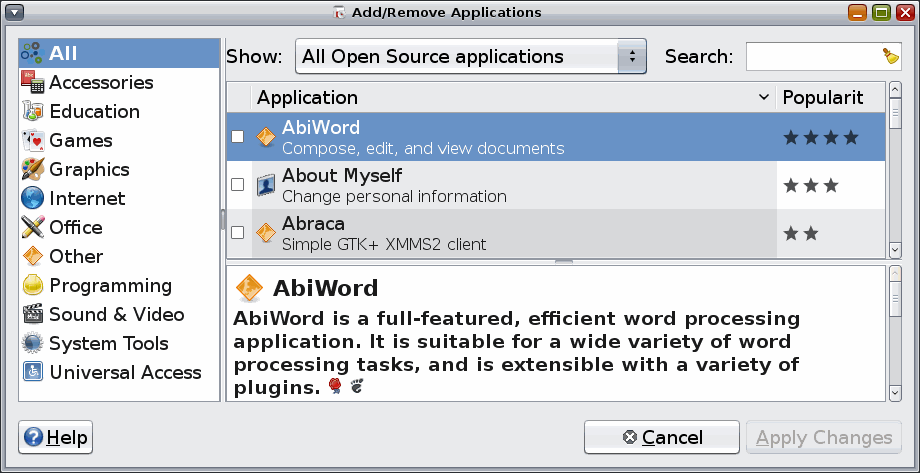
\includegraphics[width=0.6\textwidth]{ubuInstalacion1.png}
\caption{Todas las aplicaciones libres}\label{figu01}
  \end{center}
\end{figure}

Después puedes filtrar aún más utilizando la caja de texto de búsqueda con el fin de buscar el texto \codigo{Python 3} (figura~\ref{figu02}).

\begin{figure}[!h]
  \begin{center}
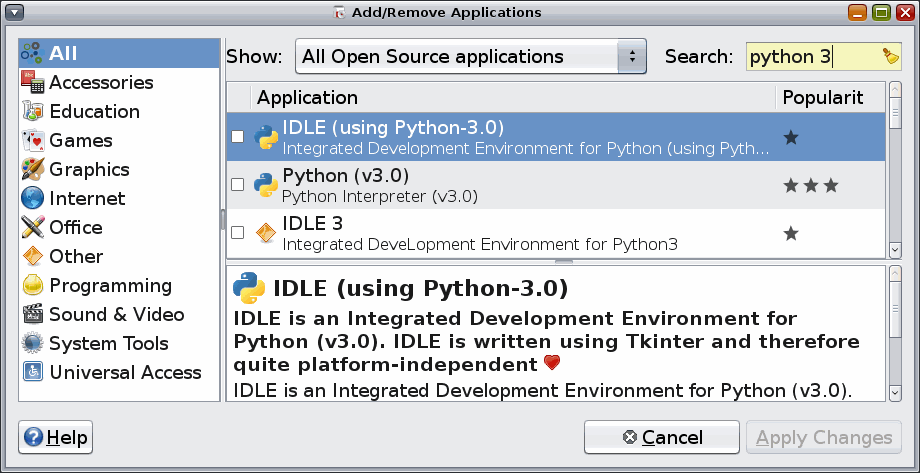
\includegraphics[width=0.6\textwidth]{ubuInstalacion2.png}
\caption{Búsqueda de aplicaciones relacionadas con Python 3}\label{figu02}
  \end{center}
\end{figure}

Ahora la lista de aplicaciones que se muestran se limita a aquellas que, de algún modo, incluyen la cadena \codigo{Python 3}. Ahora debes marcar dos paquetes. El primero es \codigo{Python (v3.0)}. Que contiene el intérprete de Python 3.

\begin{figure}[!h]
  \begin{center}
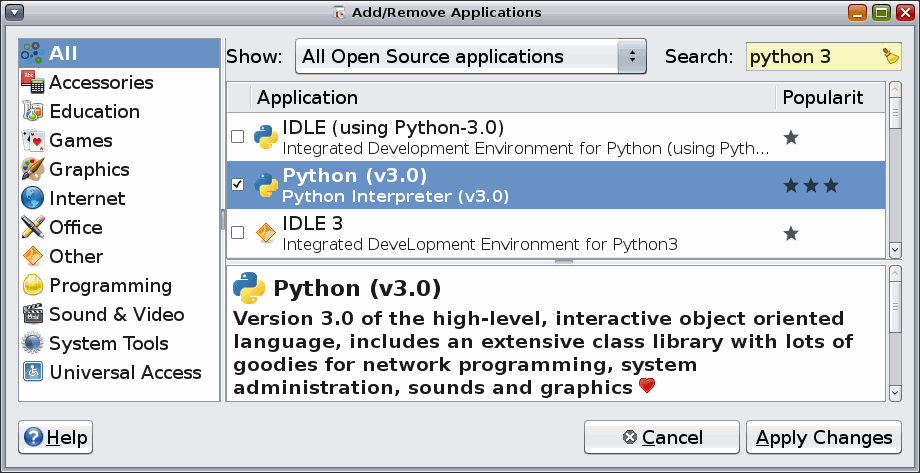
\includegraphics[width=0.6\textwidth]{ubuInstalacion3.png}
\caption{Selección del paquete Python 3}\label{figu03}
  \end{center}
\end{figure}

El segundo paquete que hay que marcar se encuentra inmediatamente delante, \codigo{IDLE (usando Python 3.0)}, que es la consola gráfica que usaremos a lo largo de todo el libro (figura~\ref{figu04}).

\begin{figure}[!h]
  \begin{center}
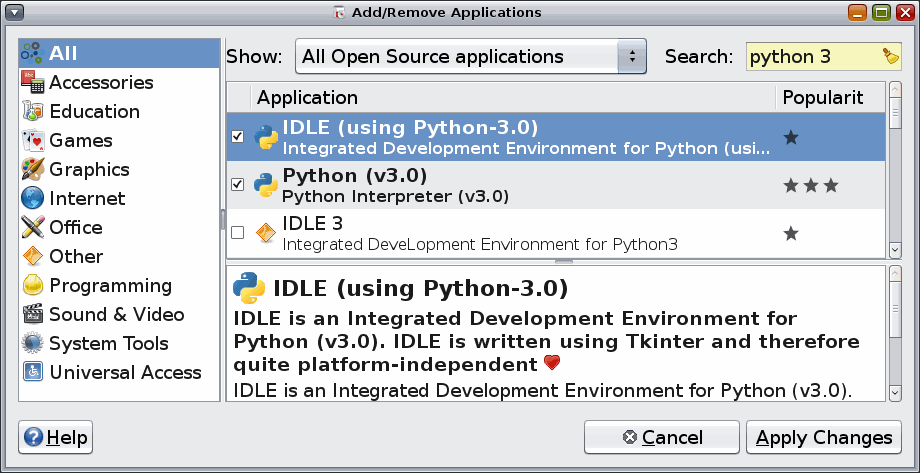
\includegraphics[width=0.6\textwidth]{ubuInstalacion4.png}
\caption{Selección del paquete IDLE}\label{figu04}
  \end{center}
\end{figure}

Una vez hayas seleccionado los dos paquetes, pulsa el botón \codigo{Aplicar cambios} para continuar.

\begin{figure}[!h]
  \begin{center}
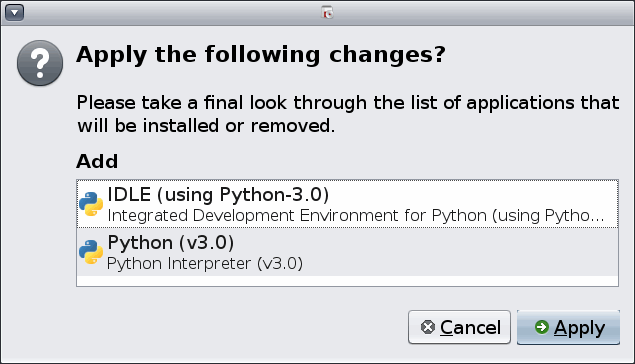
\includegraphics[width=0.6\textwidth]{ubuInstalacion5.png}
\caption{Confirmación}\label{figu05}
  \end{center}
\end{figure}

El gestor de paquetes solicitará que confirmes que quieres instalar tanto \codigo{IDLE (usando Python 3.0)} como \codigo{Python (3.0)} (figura~\ref{figu05}).

Pulsa el botón \codigo{Aplicar} para continuar.

\begin{figure}[!h]
  \begin{center}
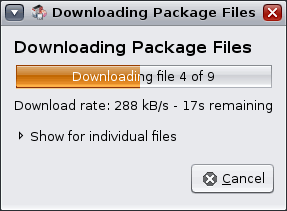
\includegraphics[width=0.5\textwidth]{ubuInstalacion6.png}
\caption{Descarga de paquetes}\label{figu06}
  \end{center}
\end{figure}

El gestor de paquetes te pedirá que te identifiques con la clave de usuario para acceder a los privilegios administrativos que permiten instalar aplicaciones. Una vez hecho esto, el gestor de paquetes mostrará una pantalla (figura~\ref{figu06}) con el grado de avance de la instalación mientras se descargan los paquetes seleccionados del repositorio de Internet de Ubuntu Linux.

\begin{figure}[!h]
  \begin{center}
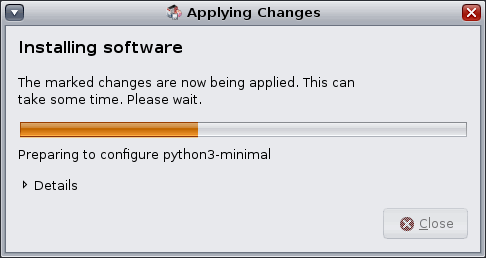
\includegraphics[width=0.5\textwidth]{ubuInstalacion7.png}
\caption{Descarga de paquetes}\label{figu07}
  \end{center}
\end{figure}

Cuando los paquetes se hayan descargado, el instalador iniciará automáticamente el proceso de instalación en tu ordenador (figura~\ref{figu07}).

\begin{figure}[!h]
  \begin{center}
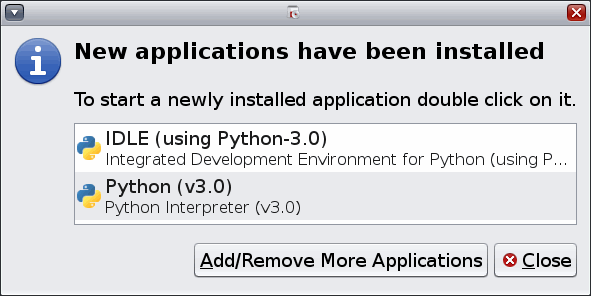
\includegraphics[width=0.5\textwidth]{ubuInstalacion8.png}
\caption{Instalación finalizada}\label{figu08}
  \end{center}
\end{figure}

Si todo va bien, el gestor de paquetes confirmará que ambos paquetes se instalaron satisfactoriamente (figura~\ref{figu08}). Desde esta pantalla puedes ejecutar directamente \codigo{IDLE} haciendo doble click sobre él. O puedes pulsar el botón \codigo{Cerrar} para finalizar el gestor de paquetes.

En cualquier caso, puedes lanzar la consola gráfica de Python siempre que quieras seleccionando \codigo{IDLE} en el submenú \codigo{Programación} del menú de \codigo{Aplicaciones}.

\begin{figure}[!h]
  \begin{center}
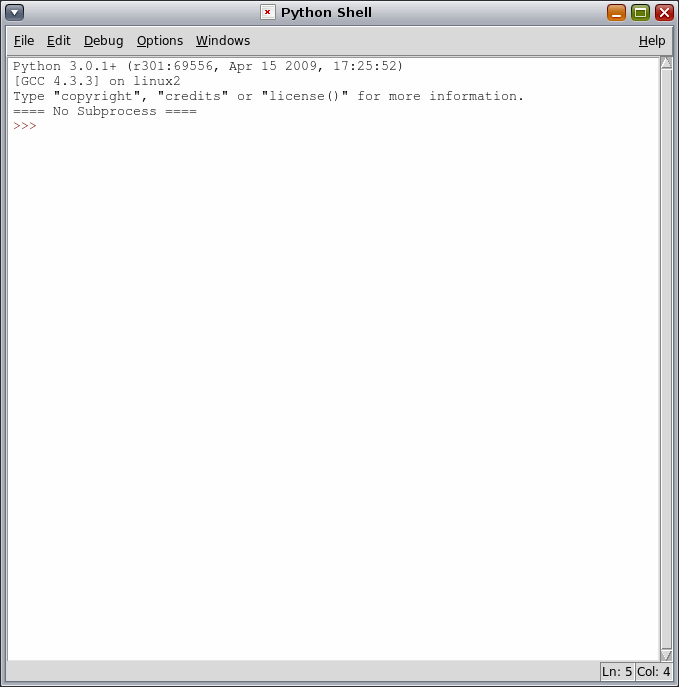
\includegraphics[width=0.5\textwidth]{ubuInstalacion9.png}
\caption{Consola de Python en Ubuntu Linux}\label{figu09}
  \end{center}
\end{figure}

Es en la consola de Python (figura~\ref{figu09}) donde pasarás la mayor parte del tiempo explorando Python. Los ejemplos de este libro asumen que eres capaz de ejecutar la consola de Python siempre que sea necesario.

Continúa en el apartado~\ref{sec:shell}

\section{Instalación en otras plataformas}

Python 3 está disponible en otras muchas plataformas. En particular, está disponible prácticamente en todas las distribuciones Linux, BSD y Sun Solaris. Por ejemplo, RedHat Linux utiliza el gestor de paquetes \codigo{yum}; FreeBSD tiene su propia colección de \href{http://www.freebsd.org/ports/}{paquetes}, y Solaris tiene el gestor de paquetes \codigo{pkgadd} y otros. Una rápida búsqueda en Internet de los términos Python 3 + emph{tu sistema operativo} te mostrará si existe un paquete de Python 3 disponible para tu sistema, y cómo instalarlo.

\section{Uso de la consola interactiva de Python}\label{sec:shell}

En la consola interactiva de Python puedes explorar la sintaxis del lenguaje, solicitar ayuda interactiva sobre las sentencias del lenguaje, y depurar programas cortos.

La consola gráfica (denominada \codigo{IDLE}) también proporciona un editor de textos bastante decente que resalta mediante colores la sintaxis del lenguaje Python. Si no tienes aún un editor de textos de tu elección, puedes darle una oportunidad a \codigo{IDLE}.

¡Vamos a comenzar! La shell de Python es un estupendo lugar para comenzar a \emph{jugar} con el lenguaje Python de forma interactiva.  A lo largo de este libro verás un montón de ejemplos como este:

\begin{listing}
\begin{verbatim}
>>> 1 + 1
2
\end{verbatim}
\end{listing}

Los tres símbolos de \emph{mayor que}, \codigo{$>>>$}, representan el \emph{prompt}\footnote{Nota del Traductor: El prompt es el indicador que usa una consola, en este caso la consola de Python, para que el usuario sepa que puede teclear alguna sentencia. Como el uso de la palabra \emph{prompt} está tan extendido para este concepto, y no existe uno en español de amplio uso, en este libro se utilizará sin traducir.} de Python. No teclees nunca estos tres caracteres. Se muestran para que sepas que este ejemplo se debe teclear en la consola de Python.

Lo que tienes que teclear es \codigo{1 + 1}.  En la consola puedes teclear cualquier expresión o sentencia válida del lenguaje. ¡No seas tímido, no muerde! Lo peor que puede pasarte es que Python muestre un mensaje de error, si tecleas algo que no entiende. Las sentencias se ejecutan inmediatamente (después de que pulses la tecla \codigo{INTRO}); las expresiones se calculan en el momento, y la consola imprime en pantalla el resultado.

\codigo{2} es el resultado de la expresión. Como \codigo{1 + 1} es una expresión válida en el lenguaje Python, al pulsar la tecla \codigo{INTRO} Python evalúa la expresióne imprime el resultado, que en este caso es \codigo{2}.

Vamos a probar otro ejemplo.

\begin{listing}
\begin{verbatim}
>>> print('¡Hola mundo!')
¡Hola mundo!
\end{verbatim}
\end{listing}

Muy sencillo, ¿no?

Pero hay muchas otras cosas que puedes hacer en la consola de Python. Si en algún momento te bloqueas ---no recuerdas una sentencia, o no recuerdas los argumentos que debes pasar a una función determinada--- puedes obtener ayuda en la propia consola. Simplemente teclea \codigo{help} y pulsa \codigo{ENTER}.

\begin{listing}
\begin{verbatim}
>>> help
Type help() for interactive help, or help(object) for help about object.
\end{verbatim}
\end{listing}

Exiten dos modos de ayuda:
\begin{itemize}
\item Puedes solicitar ayuda de un objeto concreto, lo que muestra la documentación del mismo y vuelve al \codigo{prompt} de la consola de Python. 
\item También puedes entrar en el \emph{modo ayuda}, en el que en lugar de evaluar expresiones de Python, puedes teclear palabras reservadas del lenguaje o nombres de sentencias y la consola imprime lo que sepa sobre ellas.
\end{itemize}

Para entrar en el modo interactivo de ayuda teclea \codigo{help()} y pulsa \codigo{INTRO}.

\begin{listing}
\begin{verbatim}
>>>help()

Welcome to Python 3.0!  This is the online help utility.

If this is your first time using Python, you should definitely check out
the tutorial on the Internet at http://docs.python.org/tutorial/.

Enter the name of any module, keyword, or topic to get help on writing
Python programs and using Python modules.  To quit this help utility and
return to the interpreter, just type "quit".

To get a list of available modules, keywords, or topics, type "modules",
"keywords", or "topics".  Each module also comes with a one-line summary
of what it does; to list the modules whose summaries contain a given word
such as "spam", type "modules spam".

help>
\end{verbatim}
\end{listing}

Observa que ahora el prompt cambia de \codigo{$>>>$} a \codigo{help$>$}. Este cambio sirve para recordarte que te encuentras en el modo de ayuda interactiva. Ahora puedes teclear cualquier palabra reservada, sentencia, nombre de módulo, nombre de función ---casi cualquier cosa que Python entienda--- y leer la documentación que haya disponible sobre el tema tecleado.

\begin{listing}
\begin{verbatim}
help> print

Help on built-in function print in module builtins:

print(...)
    print(value, ..., sep=' ', end='\n', file=sys.stdout)
    
    Prints the values to a stream, or to sys.stdout by default.
    Optional keyword arguments:
    file: a file-like object (stream); defaults to the current sys.stdout.
    sep:  string inserted between values, default a space.
    end:  string appended after the last value, default a newline.
help> Papaya
no Python documentation found for 'Papaya'
\end{verbatim}
\end{listing}
\begin{listing}
\begin{verbatim}
help> quit

You are now leaving help and returning to the Python interpreter.
If you want to ask for help on a particular object directly from the
interpreter, you can type "help(object)".  Executing "help('string')"
has the same effect as typing a particular string at the help> prompt.

>>>
\end{verbatim}
\end{listing}

En el ejemplo anterior se obtiene en primer lugar la documentación sobre la función print. Para ello se ha tecleado en el modo ayuda la palabra \codigo{print} y luego se ha pulsado \codigo{INTRO}. Como resultado se obtiene un texto en el que se muestra el nombre de la función, un breve resumen de la misma, los argumentos de la función y sus valores por defecto. Si la documentación te parece demasiado opaca, no te asustes. Aprenderás lo necesario sobre todos estos conceptos en los próximos capítulos de este libro.

Evidentemente el modo de ayuda no lo sabe todo. Si tecleas algo que no sea una sentencia, módulo, función u otra palabra reservada de Python,el modo de ayuda interactiva mostrará un mensaje indicando que no encuentra documentación alguna para el concepto que hayas tecleado.

Por último, para salir del modo de ayuda únicamente tienes que teclear \codigo{quit} y pulsar \codigo{INTRO}.

El prompt vuelve de nuevo a \codigo{$>>>$} para indicar que has abandonado el modo de ayuda interactiva y que de nuevo te encuentras en la consola de Python.

\codigo{IDLE}, además de servir como consola gráfica de Python, incluye también un editor de textos que conoce el lenguaje Python. Verás cómo usarlo en la sección siguiente.

\section{Editores de texto e IDEs para Python}

\codigo{IDLE} no es el único entorno existente para escribir programas en Python. Aunque es muy útil para comenzar a aprender el lenguaje, muchos desarrolladores prefieren utilizar otros editores de texto o \emph{Entornos Integrados de Desarrollo}\footnote{En inglés se suele hablar de \codigo{IDE}, para referirse a los \emph{Integrated Development Environment}, que son aplicaciones que permiten desarrollar de forma rápida al incluir un editor de textos, compilador, depurador e incluso herramientas de diseño de aplicaciones avanzadas.}. No los voy a abarcar aquí, únicamente comentaré que la comunidad de Python mantiene una lista de \href{http://wiki.python.org/moin/PythonEditors}{editores para el lenguaje Python} sobre diversas plataformas y licencias de software.

También puede ser de interés para ti la lista de \href{http://wiki.python.org/moin/IntegratedDevelopmentEnvironments}{Entornos Integrados de Desarrollo} para Python, aunque aún son pocos los que sirven para Python 3. Uno de ellos es \href{http://pydev.sourceforge.net/}{PyDev}, un plugin para \href{http://eclipse.org/}{Eclipse} que convierte a Eclipse en un completo Entorno Integrado de Desarrollo para Python. Ambos, Eclipse y PyDev, son multiplataforma y de código abierto.

Por la parte comercial, existe un entorno de desarrollo denominado \href{http://www.activestate.com/komodo/}{Komodo IDE}. Tiene una licencia que se paga por cada usuario, pero también ofrece descuento para estudiantes, y una versión con licencia de prueba limitada.

Llevo programando en Python nueve años, yo, para editar los programas, utilizo \href{http://www.gnu.org/software/emacs/}{GNU Emacs} y los depuro en la shell de línea de comando\footnote{Nota del Traductor:En mi caso uso \href{http://www.vim.org}{GVim} y el depurador de consola \href{http://pypi.python.org/pypi/pudb}{pudb}}. No existe un modo correcto de desarrollar en Python. ¡Encuentra lo que mejor se adapte a ti!

